\documentclass[11pt]{article}
\usepackage{amsmath,amsthm,amssymb}
\usepackage[colorlinks]{hyperref}
\usepackage{tikz}
\usepackage{pgfplots}
\pgfplotsset{compat=1.17}

\begin{document}
\title{Quick answer key to Recitation 6}
\author{ChatGPT 4o}
\date{23 September 2024}
\maketitle

Use the table of contents below to skip to a specific part
without seeing spoilers to the other parts.

I just used ChatGPT to write this one quickly.
ChatGPT can make mistakes, so if you spot anything that's wrong, flag me to ask.

\tableofcontents



\newpage

\section{Solution}

We are asked to convert the following points between Cartesian and polar coordinates.

\subsection{Part 1: Convert $(x, y) = (-\sqrt{3}, 1)$ to polar coordinates}

Given \( (x, y) = (-\sqrt{3}, 1) \), we convert to polar coordinates using the formulas:
\[
r = \sqrt{x^2 + y^2}, \quad \theta = \tan^{-1}\left( \frac{y}{x} \right)
\]

First, we compute the modulus \( r \):
\[
r = \sqrt{(-\sqrt{3})^2 + 1^2} = \sqrt{3 + 1} = \sqrt{4} = 2
\]

Next, we compute the argument \( \theta \):
\[
\theta = \tan^{-1}\left( \frac{1}{-\sqrt{3}} \right)
\]

Since \( x = -\sqrt{3} \) and \( y = 1 \), the point lies in the second quadrant. We first compute the reference angle:
\[
\tan^{-1}\left( \frac{1}{\sqrt{3}} \right) = \frac{\pi}{6}
\]
Thus, the argument is:
\[
\theta = \pi - \frac{\pi}{6} = \frac{5\pi}{6}
\]

Therefore, the polar coordinates are:
\[
(r, \theta) = (2, \frac{5\pi}{6})
\]

\newpage

\subsection{Part 2: Convert \( (r, \theta) = (3, \pi/6) \) to Cartesian coordinates}

Given \( (r, \theta) = (3, \pi/6) \), we convert to Cartesian coordinates using the formulas:
\[
x = r \cos\theta, \quad y = r \sin\theta
\]

First, we compute \( x \):
\[
x = 3 \cos\left( \frac{\pi}{6} \right) = 3 \times \frac{\sqrt{3}}{2} = \frac{3\sqrt{3}}{2}
\]

Next, we compute \( y \):
\[
y = 3 \sin\left( \frac{\pi}{6} \right) = 3 \times \frac{1}{2} = \frac{3}{2}
\]

Thus, the Cartesian coordinates are:
\[
(x, y) = \left( \frac{3\sqrt{3}}{2}, \frac{3}{2} \right)
\]

\newpage

\subsection{Part 3: Convert \( (x, y) = (-\sqrt{6}, -\sqrt{2}) \) to polar coordinates}

Given \( (x, y) = (-\sqrt{6}, -\sqrt{2}) \), we use the same formulas as in Part 1.

First, we compute \( r \):
\[
r = \sqrt{(-\sqrt{6})^2 + (-\sqrt{2})^2} = \sqrt{6 + 2} = \sqrt{8} = 2\sqrt{2}
\]

Next, we compute \( \theta \):
\[
\theta = \tan^{-1}\left( \frac{-\sqrt{2}}{-\sqrt{6}} \right) = \tan^{-1}\left( \frac{\sqrt{2}}{\sqrt{6}} \right) = \tan^{-1}\left( \frac{1}{\sqrt{3}} \right)
\]

The reference angle is \( \frac{\pi}{6} \). Since both \( x \) and \( y \) are negative, the point lies in the third quadrant, so:
\[
\theta = \pi + \frac{\pi}{6} = \frac{7\pi}{6}
\]

Therefore, the polar coordinates are:
\[
(r, \theta) = \left( 2\sqrt{2}, \frac{7\pi}{6} \right)
\]




\newpage

\section{Solution}

\subsection{Part 1: Show that \( \sin(\theta) = \frac{1}{2i}(e^{i\theta} - e^{-i\theta}) \)}

We start with Euler's formula:
\[
e^{i\theta} = \cos(\theta) + i\sin(\theta), \quad e^{-i\theta} = \cos(\theta) - i\sin(\theta)
\]

Subtract the second equation from the first:
\[
e^{i\theta} - e^{-i\theta} = (\cos(\theta) + i\sin(\theta)) - (\cos(\theta) - i\sin(\theta)) = 2i\sin(\theta)
\]

Solving for \( \sin(\theta) \), we get:
\[
\sin(\theta) = \frac{e^{i\theta} - e^{-i\theta}}{2i}
\]

Thus, we have shown that:
\[
\sin(\theta) = \frac{1}{2i}(e^{i\theta} - e^{-i\theta})
\]

\newpage

\subsection{Part 2: Show that \( \cos(\theta) = \frac{1}{2}(e^{i\theta} + e^{-i\theta}) \)}

Starting again with Euler's formula:
\[
e^{i\theta} = \cos(\theta) + i\sin(\theta), \quad e^{-i\theta} = \cos(\theta) - i\sin(\theta)
\]

Add the two equations:
\[
e^{i\theta} + e^{-i\theta} = (\cos(\theta) + i\sin(\theta)) + (\cos(\theta) - i\sin(\theta)) = 2\cos(\theta)
\]

Solving for \( \cos(\theta) \), we get:
\[
\cos(\theta) = \frac{e^{i\theta} + e^{-i\theta}}{2}
\]

Thus, we have shown that:
\[
\cos(\theta) = \frac{1}{2}(e^{i\theta} + e^{-i\theta})
\]

\newpage

\subsection{Part 3: Express \( \sin^3(\theta) \) in terms of \( \sin(3\theta) \) and \( \sin(\theta) \)}

We can express \( \sin^3(\theta) \) using the exponential form of \( \sin(\theta) \):
\[
\sin(\theta) = \frac{1}{2i}(e^{i\theta} - e^{-i\theta})
\]
Thus:
\[
\sin^3(\theta) = \left( \frac{1}{2i}(e^{i\theta} - e^{-i\theta}) \right)^3 = \frac{1}{(2i)^3}(e^{i\theta} - e^{-i\theta})^3
\]

Now, expand \( (e^{i\theta} - e^{-i\theta})^3 \) using the binomial theorem:
\[
(e^{i\theta} - e^{-i\theta})^3 = e^{3i\theta} - 3e^{i\theta} + 3e^{-i\theta} - e^{-3i\theta}
\]

Thus:
\[
\sin^3(\theta) = \frac{1}{-8i}(e^{3i\theta} - 3e^{i\theta} + 3e^{-i\theta} - e^{-3i\theta})
\]

We separate this expression into two parts:
\[
\sin^3(\theta) = \frac{1}{8} \left( \frac{1}{i}(e^{3i\theta} - e^{-3i\theta}) \right) - \frac{3}{8i}(e^{i\theta} - e^{-i\theta})
\]

Using the identity for \( \sin(\theta) \), we can express this as:
\[
\sin^3(\theta) = \frac{1}{4} \sin(3\theta) - \frac{3}{4} \sin(\theta)
\]

Thus, we have:
\[
\sin^3(\theta) = \frac{1}{4} \sin(3\theta) - \frac{3}{4} \sin(\theta)
\]




\newpage

\section{Solution}

We are given the complex function:
\[
f(t) = \frac{t + 2i}{1 - 3i}
\]
where \( t \) is a real number. We are asked to find the real and imaginary parts of \( f(t) \), as well as \( \overline{f(t)} \) and \( |f(t)|^2 \).

\subsection{Part 1: Find the real and imaginary parts of \( f(t) \)}

To find the real and imaginary parts of \( f(t) \), we first simplify the expression by multiplying the numerator and denominator by the complex conjugate of the denominator \( 1 - 3i \), which is \( 1 + 3i \):
\[
f(t) = \frac{t + 2i}{1 - 3i} \times \frac{1 + 3i}{1 + 3i} = \frac{(t + 2i)(1 + 3i)}{(1 - 3i)(1 + 3i)}
\]

First, simplify the denominator:
\[
(1 - 3i)(1 + 3i) = 1^2 - (3i)^2 = 1 - (-9) = 1 + 9 = 10
\]

Next, expand the numerator:
\[
(t + 2i)(1 + 3i) = t(1 + 3i) + 2i(1 + 3i) = t + 3ti + 2i + 6i^2
\]
Since \( i^2 = -1 \), this becomes:
\[
t + 3ti + 2i - 6 = (t - 6) + (3t + 2)i
\]

Thus, we have:
\[
f(t) = \frac{(t - 6) + (3t + 2)i}{10}
\]

We can now separate the real and imaginary parts:
\[
f(t) = \frac{t - 6}{10} + \frac{3t + 2}{10}i
\]

Therefore, the real and imaginary parts of \( f(t) \) are:
\[
\text{Re}(f(t)) = \frac{t - 6}{10}, \quad \text{Im}(f(t)) = \frac{3t + 2}{10}
\]

\newpage

\subsection{Part 2: Find \( \overline{f(t)} \) and \( |f(t)|^2 \)}

The complex conjugate \( \overline{f(t)} \) is obtained by changing the sign of the imaginary part:
\[
\overline{f(t)} = \frac{t - 6}{10} - \frac{3t + 2}{10}i
\]

Next, we compute \( |f(t)|^2 \), which is given by:
\[
|f(t)|^2 = f(t) \cdot \overline{f(t)} = \left( \frac{t - 6}{10} + \frac{3t + 2}{10}i \right) \left( \frac{t - 6}{10} - \frac{3t + 2}{10}i \right)
\]

Using the identity \( (a + bi)(a - bi) = a^2 + b^2 \), we get:
\[
|f(t)|^2 = \left( \frac{t - 6}{10} \right)^2 + \left( \frac{3t + 2}{10} \right)^2
\]
\[
= \frac{(t - 6)^2}{100} + \frac{(3t + 2)^2}{100}
\]
\[
= \frac{(t - 6)^2 + (3t + 2)^2}{100}
\]

Now, expand the terms:
\[
(t - 6)^2 = t^2 - 12t + 36, \quad (3t + 2)^2 = 9t^2 + 12t + 4
\]

Adding them together:
\[
(t - 6)^2 + (3t + 2)^2 = t^2 - 12t + 36 + 9t^2 + 12t + 4 = 10t^2 + 40
\]

Thus:
\[
|f(t)|^2 = \frac{10t^2 + 40}{100} = \frac{t^2 + 4}{10}
\]




\newpage

\section{Solution}

We are tasked with finding the fourth powers of \( 2 + 2i \) and \( -3 + i\sqrt{3} \) using their polar forms. Afterward, we will graph these numbers and their fourth powers on the complex plane.

\subsection{Part 1: Fourth power of \( 2 + 2i \)}

First, we express \( 2 + 2i \) in polar form. The modulus \( r \) of \( 2 + 2i \) is:
\[
r = |2 + 2i| = \sqrt{2^2 + 2^2} = \sqrt{4 + 4} = \sqrt{8} = 2\sqrt{2}
\]

Next, we compute the argument \( \theta \):
\[
\theta = \arg(2 + 2i) = \tan^{-1}\left( \frac{2}{2} \right) = \frac{\pi}{4}
\]

Thus, the polar form of \( 2 + 2i \) is:
\[
2 + 2i = 2\sqrt{2} \left( \cos\frac{\pi}{4} + i \sin\frac{\pi}{4} \right)
\]

To find the fourth power, we use De Moivre's theorem:
\[
(2 + 2i)^4 = \left( 2\sqrt{2} \right)^4 \left( \cos\left( 4 \times \frac{\pi}{4} \right) + i \sin\left( 4 \times \frac{\pi}{4} \right) \right)
\]
\[
= (2\sqrt{2})^4 \left( \cos\pi + i \sin\pi \right)
\]
\[
= 64(-1) = -64
\]

Thus, the fourth power of \( 2 + 2i \) is \( -64 \).

\newpage

\subsection{Part 2: Fourth power of \( -3 + i\sqrt{3} \)}

Next, we express \( -3 + i\sqrt{3} \) in polar form. The modulus \( r \) is:
\[
r = |-3 + i\sqrt{3}| = \sqrt{(-3)^2 + (\sqrt{3})^2} = \sqrt{9 + 3} = \sqrt{12} = 2\sqrt{3}
\]

The argument \( \theta \) is:
\[
\theta = \arg(-3 + i\sqrt{3}) = \pi - \tan^{-1}\left( \frac{\sqrt{3}}{3} \right) = \pi - \frac{\pi}{6} = \frac{5\pi}{6}
\]

Thus, the polar form of \( -3 + i\sqrt{3} \) is:
\[
-3 + i\sqrt{3} = 2\sqrt{3} \left( \cos\frac{5\pi}{6} + i \sin\frac{5\pi}{6} \right)
\]

Now, we find the fourth power using De Moivre's theorem:
\[
(-3 + i\sqrt{3})^4 = \left( 2\sqrt{3} \right)^4 \left( \cos\left( 4 \times \frac{5\pi}{6} \right) + i \sin\left( 4 \times \frac{5\pi}{6} \right) \right)
\]
\[
= (2\sqrt{3})^4 \left( \cos\frac{10\pi}{3} + i \sin\frac{10\pi}{3} \right)
\]
Since \( \frac{10\pi}{3} = 2\pi + \frac{4\pi}{3} \), we simplify to:
\[
(-3 + i\sqrt{3})^4 = 144 \left( \cos\frac{4\pi}{3} + i \sin\frac{4\pi}{3} \right)
\]
\[
= 144 \left( -\frac{1}{2} - i\frac{\sqrt{3}}{2} \right) = -72 - 72i\sqrt{3}
\]

Thus, the fourth power of \( -3 + i\sqrt{3} \) is \( -72 - 72i\sqrt{3} \).

\newpage

\subsection{Part 3: Graphing the numbers and their fourth powers}

The following plot shows the numbers \( 2 + 2i \) and \( -3 + i\sqrt{3} \), along with their fourth powers, \( -64 \) and \( -72 - 72i\sqrt{3} \), respectively.

\begin{center}
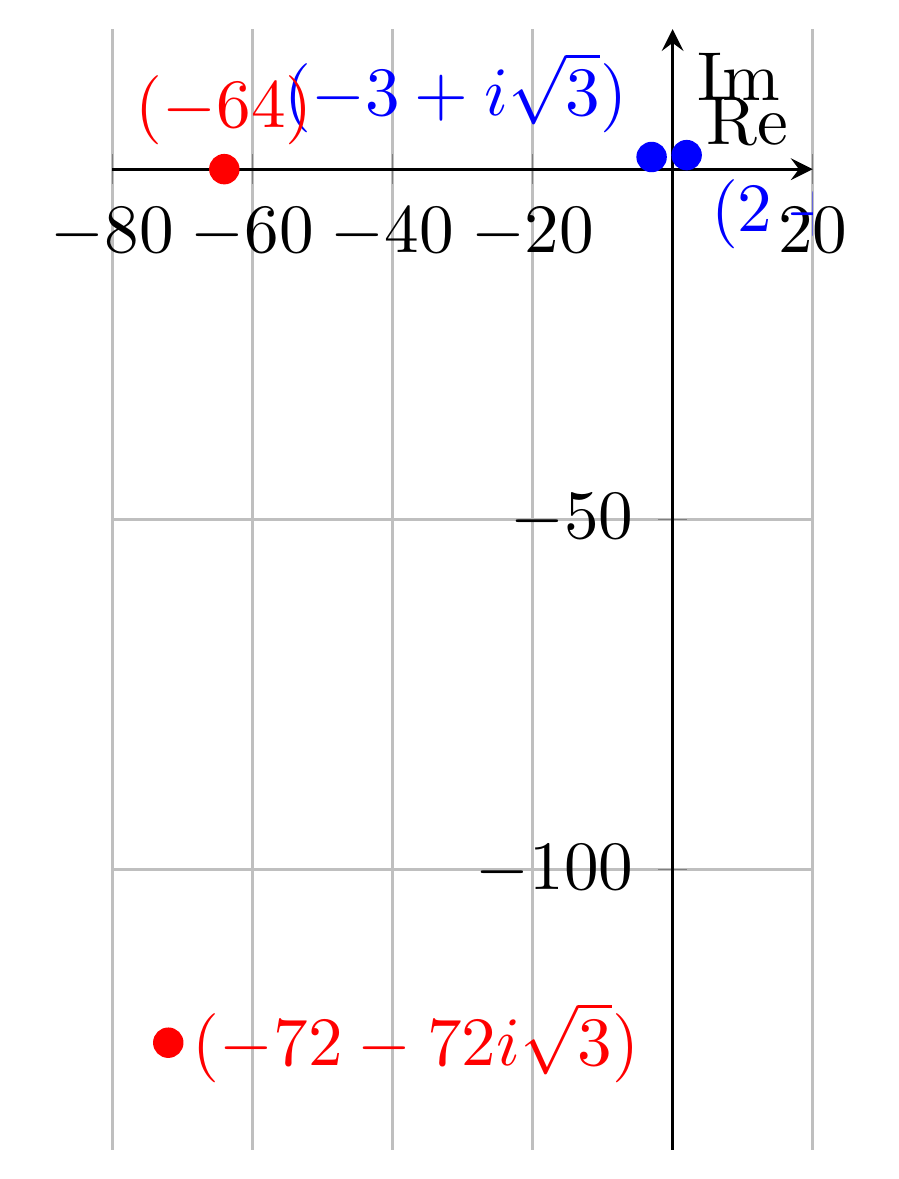
\begin{tikzpicture}[scale=2.5]
    \begin{axis}[
        axis lines = middle,
        xlabel = {Re},
        ylabel = {Im},
        grid = both,
        xmin = -80, xmax = 20,
        ymin = -140, ymax = 20,
        axis equal image
    ]
    % Plot original points
    \addplot[only marks, blue] coordinates {(2, 2)} node[below right] {$(2 + 2i)$};
    \addplot[only marks, blue] coordinates {(-3, 1.732)} node[above left] {$(-3 + i\sqrt{3})$};

    % Plot fourth powers
    \addplot[only marks, red] coordinates {(-64, 0)} node[above] {$(-64)$};
    \addplot[only marks, red] coordinates {(-72, -72*1.732)} node[right] {$(-72 - 72i\sqrt{3})$};

    \end{axis}
\end{tikzpicture}
\end{center}




\newpage

\section{Solution}

We are tasked with finding the complex eigenvalues and eigenvectors of the matrix:
\[
A = \begin{pmatrix} 0 & -1 \\ 1 & 0 \end{pmatrix}
\]

\newpage

\subsection{Step 1: Find the characteristic polynomial}

The eigenvalues are solutions to the characteristic equation:
\[
\det(A - \lambda I) = 0
\]
where \( I \) is the identity matrix and \( \lambda \) is the eigenvalue. First, compute \( A - \lambda I \):
\[
A - \lambda I = \begin{pmatrix} 0 & -1 \\ 1 & 0 \end{pmatrix} - \lambda \begin{pmatrix} 1 & 0 \\ 0 & 1 \end{pmatrix} = \begin{pmatrix} -\lambda & -1 \\ 1 & -\lambda \end{pmatrix}
\]

Now, compute the determinant of this matrix:
\[
\det(A - \lambda I) = \det\begin{pmatrix} -\lambda & -1 \\ 1 & -\lambda \end{pmatrix} = (-\lambda)(-\lambda) - (-1)(1)
\]
\[
= \lambda^2 - 1
\]

Thus, the characteristic equation is:
\[
\lambda^2 + 1 = 0
\]

Solving for \( \lambda \), we get:
\[
\lambda^2 = -1 \quad \Rightarrow \quad \lambda = \pm i
\]

Therefore, the eigenvalues are \( \lambda_1 = i \) and \( \lambda_2 = -i \).

\newpage

\subsection{Step 2: Find the eigenvectors}

For each eigenvalue, we solve the system \( (A - \lambda I) \mathbf{v} = 0 \) where \( \mathbf{v} = \begin{pmatrix} v_1 \\ v_2 \end{pmatrix} \) is the eigenvector.

\paragraph{Eigenvalue \( \lambda_1 = i \):}

We solve:
\[
(A - iI) \mathbf{v} = \begin{pmatrix} -i & -1 \\ 1 & -i \end{pmatrix} \begin{pmatrix} v_1 \\ v_2 \end{pmatrix} = \begin{pmatrix} 0 \\ 0 \end{pmatrix}
\]

This gives the system of equations:
\[
-iv_1 - v_2 = 0 \quad \text{(1)}
\]
\[
v_1 - iv_2 = 0 \quad \text{(2)}
\]

From equation (2), solve for \( v_1 \):
\[
v_1 = iv_2
\]

Substitute \( v_1 = iv_2 \) into equation (1):
\[
-i(iv_2) - v_2 = 0 \quad \Rightarrow \quad v_2 + v_2 = 0 \quad \Rightarrow \quad v_2 = 0
\]

If \( v_2 = 0 \), then from equation (2), \( v_1 = 0 \), but this would not provide a valid eigenvector. Thus, assume \( v_2 = 1 \), which implies \( v_1 = i \).

Therefore, the eigenvector corresponding to \( \lambda_1 = i \) is:
\[
\mathbf{v}_1 = \begin{pmatrix} i \\ 1 \end{pmatrix}
\]

\paragraph{Eigenvalue \( \lambda_2 = -i \):}

We solve:
\[
(A + iI) \mathbf{v} = \begin{pmatrix} i & -1 \\ 1 & i \end{pmatrix} \begin{pmatrix} v_1 \\ v_2 \end{pmatrix} = \begin{pmatrix} 0 \\ 0 \end{pmatrix}
\]

This gives the system of equations:
\[
iv_1 - v_2 = 0 \quad \text{(3)}
\]
\[
v_1 + iv_2 = 0 \quad \text{(4)}
\]

From equation (4), solve for \( v_1 \):
\[
v_1 = -iv_2
\]

Substitute \( v_1 = -iv_2 \) into equation (3):
\[
i(-iv_2) - v_2 = 0 \quad \Rightarrow \quad v_2 + v_2 = 0 \quad \Rightarrow \quad v_2 = 0
\]

If \( v_2 = 0 \), this would lead to \( v_1 = 0 \), which is not a valid eigenvector. Therefore, assume \( v_2 = 1 \), which gives \( v_1 = -i \).

Thus, the eigenvector corresponding to \( \lambda_2 = -i \) is:
\[
\mathbf{v}_2 = \begin{pmatrix} -i \\ 1 \end{pmatrix}
\]

\newpage

\subsection{Conclusion}

The eigenvalues of the matrix \( A = \begin{pmatrix} 0 & -1 \\ 1 & 0 \end{pmatrix} \) are:
\[
\lambda_1 = i, \quad \lambda_2 = -i
\]
The corresponding eigenvectors are:
\[
\mathbf{v}_1 = \begin{pmatrix} i \\ 1 \end{pmatrix}, \quad \mathbf{v}_2 = \begin{pmatrix} -i \\ 1 \end{pmatrix}
\]


\end{document}
